\documentclass[aspectratio=169,dvipsnames]{beamer}
\usepackage[utf8]{inputenc}
\usepackage[english]{babel}
\usepackage{graphicx,hyperref,icmc,url}
\usepackage{subcaption}
\usepackage{multirow}
\usepackage{minted}
\usepackage{listings}
\usepackage{tikz}
\usepackage{array}
\usepackage{xcolor, soul}  
\usepackage{mathtools}

\usepackage{fontawesome5}




\usepackage{listings}% http://ctan.org/pkg/listings
\usepackage{graphbox}
\usepackage{booktabs}
\usetikzlibrary{positioning}

\newcommand{\destaq}[1]{\textcolor{BlueViolet}{\textbf{#1}}}
\newcommand\todo[1]{\colorbox{green}{#1}}

\definecolor{echodrk}{HTML}{0099cc}
\definecolor{olivegreen}{rgb}{0,0.6,0}
\definecolor{camdrk}{RGB}{0,62,114}

\usetikzlibrary{arrows,shapes}

\definecolor{mygreen}{rgb}{0,0.6,0}

\definecolor{mymauve}{rgb}{0.58,0,0.82} 

\usetikzlibrary{arrows,shapes, decorations.pathmorphing,backgrounds,positioning}

\pgfdeclarelayer{background}
\pgfsetlayers{background,main}

\tikzstyle{vertex}=[circle,fill=black!25,minimum size=20pt,inner sep=0pt]
\tikzstyle{selected vertex} = [vertex, fill=red!24]
\tikzstyle{select vertex} = [vertex, fill=blue!24]
\tikzstyle{selectx vertex} = [vertex, fill=green!24]
\tikzstyle{edge} = [draw,thick,-]
\tikzstyle{selected edge} = [draw,line width=5pt,-,red!50]


% The title of the presentation:
%  - first a short version which is visible at the bottom of each slide;
%  - second the full title shown on the title slide;
\title[Spectral GNNs vs GAT
]{Spectral GNNs vs GATs \\ When attention is (not all you need) the "only" option
}

% Optional: a subtitle to be displayed on the title slide


% The author(s) of the presentation:
%  - again first a short version to be displayed at the bottom;
%  - next the full list of authors, which may include contact information;
\author[Jorge Luiz Franco]{Jorge Luiz Franco\\ \bigskip
\textsc{Complex Networks for Computer Science}\\ \bigskip
Professor: Diego Amancio, Ph.D.}

% \\ \bigskip
    % \large{}

% The institute:
%  - to start the name of the university as displayed on the top of each slide
%    this can be adjusted such that you can also create a Dutch version
%  - next the institute information as displayed on the title slide
\institute[ICMC/USP]{Universidade de São Paulo - ICMC}

% Add a date and possibly the name of the event to the slides
%  - again first a short version to be shown at the bottom of each slide
%  - second the full date and event name for the title slide
\date[2024]{\footnotesize{Nov 3, 2024}}

\sloppy

\AtBeginSection[]
{
    \begin{frame}<beamer>{Summary}
        \tableofcontents[currentsection]
    \end{frame}
}

\begin{document}
    
    \begin{frame}[plain]
        \titlepage
    \end{frame}
    
    \begin{frame}
      \frametitle{Summary}
      \tableofcontents
    \end{frame}
    
%%%%%%%%%%%%%%%%%%%%%%%%%%%%%%%%%%%%%%%%%%%%%%%%%%%%%%%%%%%%%%%%

% Introduction
% Materials and Methods
%   Datasets
%   MST
%   OPF
% Experiments
%   Initial
%   DTW
%   Pruning and Improvements
%   Batch-Tests
%   Results
%   Difficulties, limitations, and future works

\section{Introduction}

\begin{frame}{Motivation}
\begin{itemize}
    \item Graph machine learning can be tracked backwards to the problem of `learning' on data that is inherently a graph \cite{silva2016machine, JMLR:Perozzi} or can be modeled as a graph \cite{verri2013,grape2020}
    \item Variety of tasks:  node/edge classification, link prediction, graph partitioning, which rely on learning representations from graph-structured data.
    \item  Techniques were most developed by complex networks researchers.
    \item \textbf{Last decade:} significant shift towards the merging of three main communities: graph signal processing, deep learning and complex nets.
    
\end{itemize}
\end{frame}

\begin{frame}{GraphML paradigms Overview}
    \begin{itemize}
        \item Three main learning paradigms: supervised, unsupervised, and semi-supervised learning
        \item We are interested on the (semi-)supervised learning paradigm, which encompasses a variety of techniques designed to leverage learning to (partially-)labeled data \cite{verri2018advantages,amanciof}
        \item  Focus in the subset of graph elements (nodes,edges,graph structure) prediction(classification/regression) methods.
        \item Consider the division of the field into \texttt{traditional} graph learning and \texttt{deep} graph learning
        
    \end{itemize}
    \end{frame}

\begin{frame}{Introduction to Last-Mile Delivery Drones}
    \begin{figure}
      \begin{columns}
        \column{.3\linewidth}
        \caption{Drones Congestion in a high-traffic Last Mile Delivery context. \\ Source: \cite{imageDronesCongestion}}
        \label{fig:example left}
        \column{.65\linewidth}
        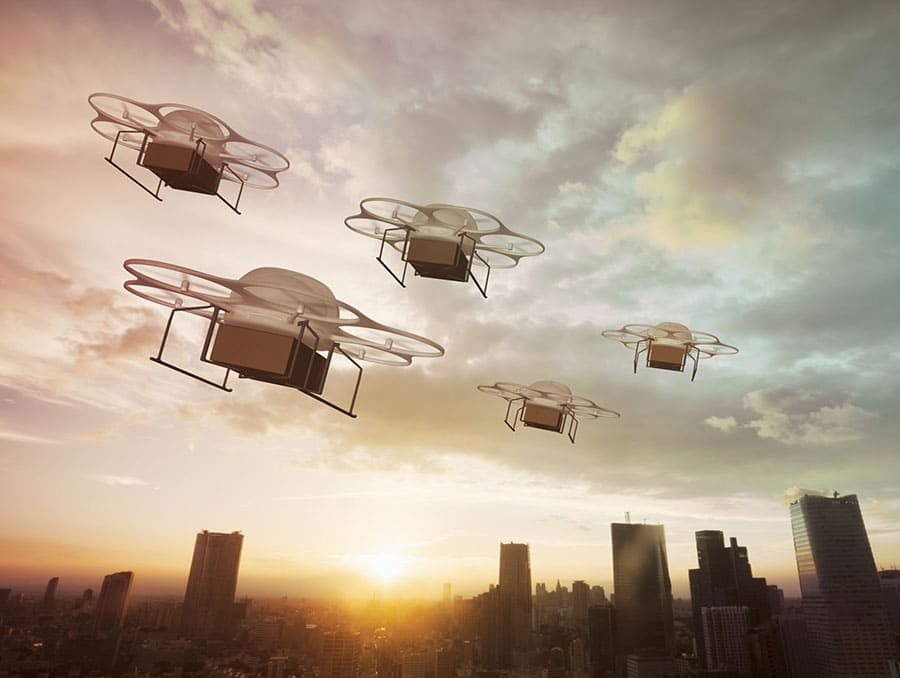
\includegraphics[width=\textwidth]{img/Drone Congestion.jpg}
      \end{columns}
    \end{figure}

\end{frame}

\begin{frame}{Introduction to Last-Mile Delivery Drones}
\destaq{Last Mile Delivery Drones (LMDD)}
\begin{itemize}
    \item Heterogeneous research area:
    \begin{itemize}
        \item Combining drones and trucks.
        \item Linear integer modeling.
        \item Fuzzy logic for uncertainties.
        \item Multi-objective optimization.
        \item Exclusive drone-based solutions.
    \end{itemize}
    \item \textbf{Complex Systems Decentralized Approach}:
    \begin{itemize}
        \item Tradable permit model for multi-agent airspace use \cite{Verri}.
    \end{itemize}
\end{itemize}

\end{frame}

\begin{frame}{Related Work and Centralized Control}
\begin{itemize}
    \item \textbf{Necessity of Air Traffic Management}:
    \begin{itemize}
        \item Most centralized models don't address collision avoidance \cite{DUKKANCI2023}.
        \item Ensuring optimal path planning and efficient airspace control.
    \end{itemize}
    \item \textbf{Centralized Control and UTM}:
    \begin{itemize}
        \item \textbf{Centralized Control}:
        \begin{itemize}
            \item Federal Aviation Administration (FAA) and NASA's Unmanned Aircraft System Traffic Management (UTM) \cite{nasa}.
            \item Ensures organized, legislative-backed airspace control.
        \end{itemize}
        \item \textbf{Decentralized Models}:
        \begin{itemize}
            \item Novel but complex in scalability and regulatory compliance.
        \end{itemize}
    \end{itemize}
\end{itemize}
\end{frame}


\begin{frame}{Proposed Approach}
\begin{itemize}
    \item \textbf{Aispace Control and MAPF Approach}:
    \begin{itemize}
        \item Multi-Agent Path Finding (MAPF) is a solution for addressing spatial characteristics and collision avoidance.
    \end{itemize}
    \item \textbf{Proposed Strategy}:
    \begin{itemize}
        \item Employing MAPF strategy for Last Mile Delivery Drone problem.
        \item Three approaches: MILP, heuristic and hybrid.
        \item Use of prioritized planning \cite{7138650} and conflict-based search \cite{SHARON201540} to manage computational complexity in the heuristic.
        \item Comparing the MILP with the heuristic.
        \item Qualitative comparison between centralized and decentralized approaches.
    \end{itemize}
\end{itemize}
\end{frame}




\section{Spectral GNNs}

\begin{frame}{Spectral GNNs}
    \destaq{Introduction to Spectral GNNs}
    \begin{itemize}
        \item Spectral Graph Neural Networks derived from GSP principles.
        \item \textbf{Key Concept}: Graph Laplacian $\mathcal{L} = D - A$ (degree matrix $D$ and adjacency matrix $A$) captures graph structure, enabling spectral operations analogous to Fourier transforms.
        \item Objective: Represent node features as signals on a graph.
        \item Spectral Methods:
        \begin{itemize}
            \item \textbf{Eigenvalue-based}: Filters created in Fourier domain.
            \item \textbf{Eigenvector-based}: Decomposition of signals via spectral basis \cite{bo2023surveyspectralgraphneural}.
        \end{itemize}
    \end{itemize}
\end{frame}

\begin{frame}{Spectral CNN (SCNN)}
    \destaq{First Spectral GNN - Spectral CNN (SCNN)}
    \begin{itemize}
        \item \textbf{Concept}: Transforms CNN concepts from images to graphs.
        \item \textbf{Mathematics}:
        \begin{itemize}
            \item Graph Fourier Transform: $\hat{f} = U^T f$
            \item Convolution: $g_{\theta} \star f = U g_{\theta} U^T f$, where $U$ and $\Lambda$ are derived from $\mathcal{L} = U \Lambda U^T$.
            \item \textbf{Challenges}:
            \begin{itemize}
                \item High computational cost $\mathcal{O}(n^3)$.
                \item Non-localized eigenvectors can overshadow local details \cite{bruna2013spectral}.
            \end{itemize}
        \end{itemize}
    \end{itemize}
\end{frame}

\begin{frame}{Graph Laplacian Spectra}
    \begin{figure}
      \begin{columns}
        \column{.3\linewidth}
        \caption{Eigenvectors as signals denotes nodal regions of eigenvalues of the graph Laplacian.}
        \label{fig:graph_spectra}
        \column{.65\linewidth}
        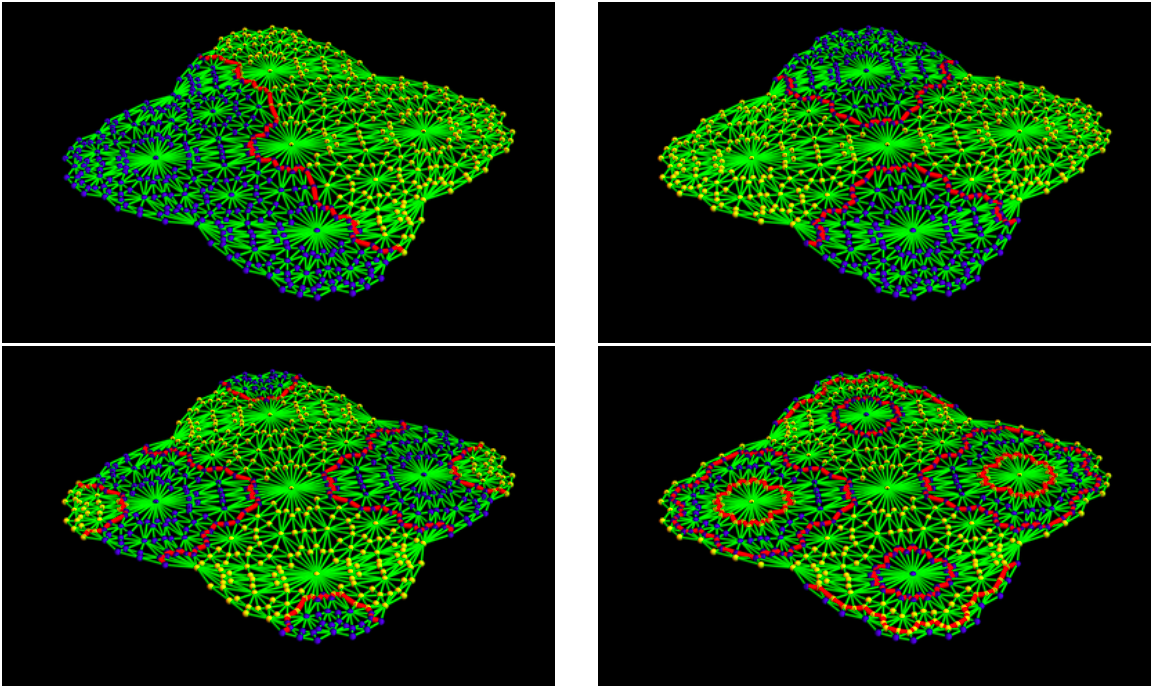
\includegraphics[width=\textwidth]{img/graph_spectra.png}
      \end{columns}
    \end{figure}

\end{frame}


\begin{frame}{ChebNet}
    \destaq{ChebNet - Addressing SCNN Limitations}
    \begin{itemize}
        \item \textbf{Introduction of Chebyshev Polynomials}:
        \begin{itemize}
            \item Approximates spectral filters for reduced computational demands using Chebyshev polynomials.
            \item Defines filters as: $ g_{\theta}(\mathcal{L} ) f = \sum_{k=0}^{K-1} \theta_k T_k(\widetilde{\mathcal{L}}) f $.
            \item Scaled Laplacian: $\widetilde{\mathcal{L}} = 2 \frac{\mathcal{L}}{\lambda_\text{max}} - I_n$.
        \end{itemize}
        \item \textbf{Advantages}:
        \begin{itemize}
            \item \textbf{Scalability}: Only first eigenpair needed ($\mathcal{O}(n^2)$ via power method).
            \item \textbf{Localized Filtering}: $K$-localized for $K^{th}$-order polynomial filters, representing paths up to length $K$ \cite{defferrard2016convolutional}.
        \end{itemize}
    \end{itemize}
\end{frame}

\begin{frame}{Graph Convolutional Networks (GCNs)}
    \destaq{Graph Convolutional Networks (GCNs) - A Simplified Approach}
    \begin{itemize}
        \item \textbf{GCN Concept}:
        \begin{itemize}
            \item Rooted in Chebyshev expansion truncation ($K=1$), focusing on first-order neighbors.
            \item Propagation Rule: $g_{\theta} \star f \approx \theta (I_n + \widetilde{A}) f$ with $\widetilde{A} = D^{-\frac{1}{2}} A D^{-\frac{1}{2}}$.
        \end{itemize}
        \item \textbf{Benefits}:
        \begin{itemize}
            \item Simplifies computation while remaining effective.
            \item Often categorized as a spatial method due to neighborhood aggregation \cite{kipf2016semi}, \cite{wu2019simplifying}.
        \end{itemize}
    \end{itemize}
\end{frame}

\begin{frame}{GCN diagram}
    \begin{figure}[h]
    \centering
    \begin{columns}

    \column{.25\linewidth}

    \caption{Graph Convolution updating node embedding $\vec{h_b}$}

    \label{fig:visualgo}

    \column{.75\linewidth}
    \resizebox{0.975\columnwidth}{0.455\linewidth}{%

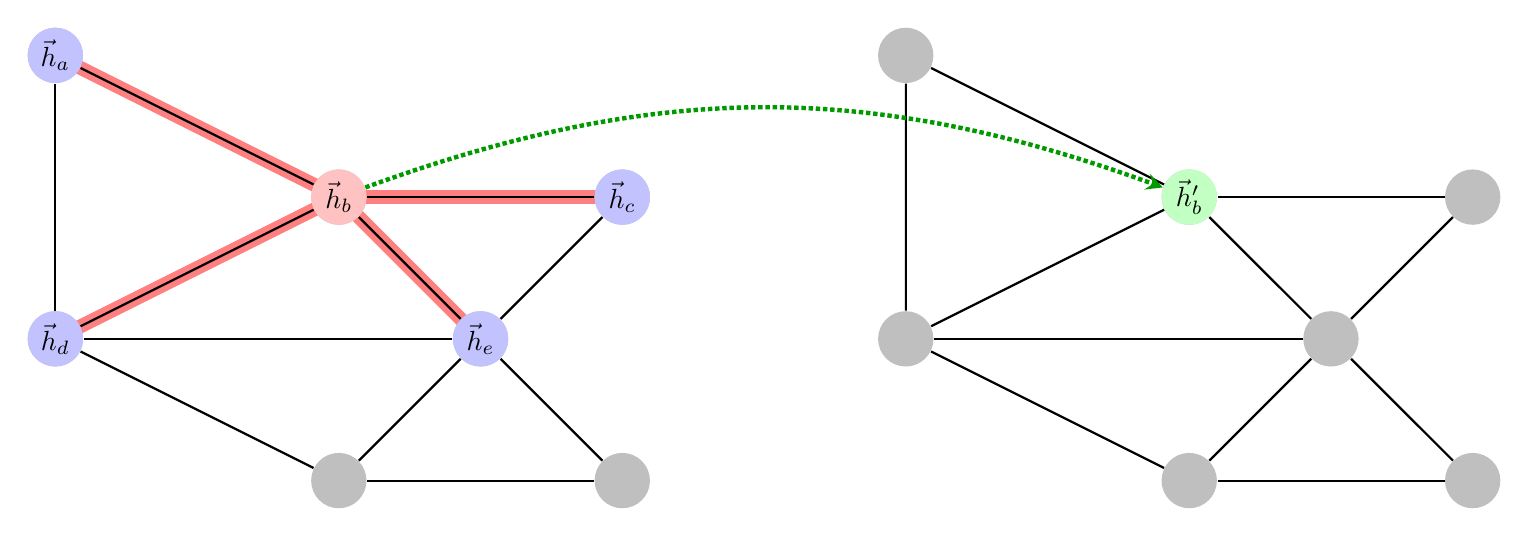
\begin{tikzpicture}[scale=1.8, auto,swap]
    \foreach \pos/\name in {{(0,2)/a}, {(2,1)/b}, {(4,1)/c},
                            {(0,0)/d}, {(3,0)/e}, {(2,-1)/f}, {(4,-1)/g}}
        \node[vertex] (\name) at \pos {};
        
    \foreach \source/ \dest /\weight in {b/a/7, c/b/8,d/a/5,d/b/9,
                                         e/b/7, e/c/5,e/d/15,
                                         f/d/6,f/e/8,
                                         g/e/9,g/f/11}
        \path[edge] (\source) -- (\dest);
         
    \foreach \vertex / \fr in {b/4}
        \path node[selected vertex] at (\vertex) {$\vec{h}_b$};
    \foreach \vertex / \fr in {a/4, c/4, d/4, e/5}
        \path node[select vertex] at (\vertex) {$\vec{h}_{\vertex}$};
    \begin{pgfonlayer}{background}
        \foreach \source / \dest in {b/c,d/b,a/b,b/e}
            \path[selected edge] (\source.center) -- (\dest.center);
    \end{pgfonlayer}
    
    \foreach \pos/\name in {{(6,2)/a1}, {(8,1)/b1}, {(10,1)/c1},
                            {(6,0)/d1}, {(9,0)/e1}, {(8,-1)/f1}, {(10,-1)/g1}}
        \node[vertex] (\name) at \pos {};
    \foreach \source/ \dest /\weight in {b1/a1/7, c1/b1/8,d1/a1/5,d1/b1/9,
                                         e1/b1/7, e1/c1/5,e1/d1/15,
                                         f1/d1/6,f1/e1/8,
                                         g1/e1/9,g1/f1/11}
        \path[edge] (\source) -- (\dest);
    \foreach \vertex / \fr in {b1/4}
        \path node[selectx vertex] at (\vertex) {$\vec{h}'_b$};
        
    \draw[-stealth, densely dotted, ultra thick, mygreen] (b) edge[bend left=20] (b1);
\end{tikzpicture}


}
\end{columns}
\end{figure}
\end{frame}

\begin{frame}{Limitations of Spectral Methods}
    \destaq{Limitations of Spectral Methods}
    \begin{itemize}
        \item Restriction: Spectral GNNs typically work only on undirected graphs as they rely on symmetric spectral decomposition.

        \item Scalability: GCNs apart, spectral methods tend to be computationally expensive for large graphs.

        \item The nature of the adjacency matrix enforces `node-centric' approaches that may not be suitable for all tasks.

    \end{itemize}
\end{frame}

\section{Spatial GNNs}


\begin{frame}{Spatial-based GNNs Overview}
    \begin{itemize}
        \item Spatial-based GNNs perform convolutions in the spatial domain by directly leveraging the graph structure.
        \item These methods aggregate features from local neighborhoods, similar to CNNs on image data.
        \item Each node's features are updated iteratively through message passing with its neighboring nodes.
        \item Suitable for large-scale graphs due to their scalability and flexibility.
    \end{itemize}
\end{frame}

\begin{frame}{Message Passing Framework for Spatial GNNs}
    \begin{itemize}
        \item At layer \( t \), each node \( i \) aggregates features from its neighbors \( \mathcal{N}(i) \).
        \[
        \mathbf{m}_i^{(t+1)} = \text{AGGREGATE}^{(t)} \left( \left\{ \mathbf{h}_j^{(t)} : j \in \mathcal{N}(i) \right\} \right)
        \]
        \item Node \( i \) then updates its own features based on the aggregated message:
        \[
        \mathbf{h}_i^{(t+1)} = \text{UPDATE}^{(t)} \left( \mathbf{h}_i^{(t)}, \mathbf{m}_i^{(t+1)} \right)
        \]
        \item Flexible, adaptable to dynamic graphs, as they only require local neighborhood information.
    \end{itemize}
\end{frame}

\begin{frame}{Message Passing Diagram}

    \begin{figure}[h]
  \centering
  \begin{columns}

    \column{.25\linewidth}

    \caption{Message Passing GNN}

    \label{fig:visualgo}

    \column{.75\linewidth}
    \resizebox{0.825\columnwidth}{0.625\linewidth}{%

      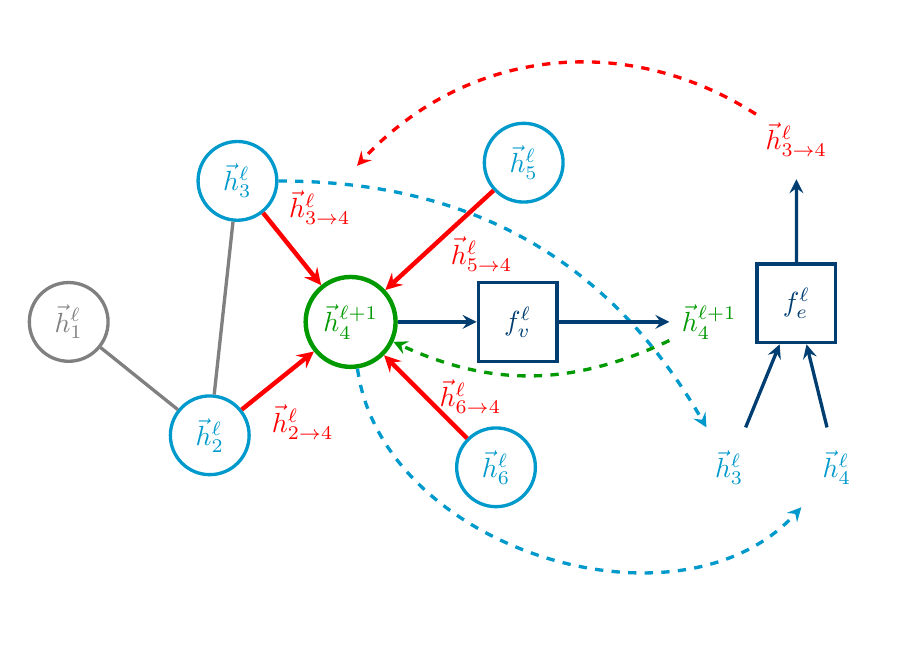
\begin{tikzpicture}[scale=.8, every node/.style={minimum size=1cm}]
        \node[circle, gray, draw, very thick] (1) {$\vec{h}^\ell_1$};
        \node[circle, echodrk, draw, below right=2em and 3em of 1, very thick] (2) {$\vec{h}^\ell_2$};
        \node[circle, draw, echodrk, above right=3em and 4em of 1, very thick] (3) {$\vec{h}^\ell_3$};
        \node[circle, draw, olivegreen, right=7em of 1, ultra thick] (4) {$\vec{h}^{\ell+1}_4$};
        \node[circle, echodrk, draw, above right=3.5em and 4em of 4, very thick] (5) {$\vec{h}^\ell_5$};
        \node[circle, echodrk, draw, below right=3em and 3em of 4, very thick] (6) {$\vec{h}^\ell_6$};

        \draw[gray, very thick] (1) -- (2);
        \draw[gray, very thick] (2) -- (3);
        \draw[red, ultra thick, -stealth] (2) -- node[below, xshift=0.9em] (ll) {$\vec{h}_{2\rightarrow 4}^\ell$} (4);
        \draw[red, ultra thick, -stealth] (3) -- node[above,xshift=1em, inner sep=0em] (l1) {$\vec{h}_{3\rightarrow 4}^\ell$} (4);
        \draw[red,ultra thick, -stealth] (5) -- node[right, yshift=-0.5em] (lr) {$\vec{h}_{5\rightarrow 4}^\ell$} (4);
        \draw[red,ultra thick, -stealth] (6) -- node[right, xshift=0.1em] (lw) {$\vec{h}_{6\rightarrow 4}^\ell$} (4);

        \node[right=5.5em of 6, echodrk] (31) {$\vec{h}^\ell_3$};
        \node[right=1em of 31, echodrk] (41) {$\vec{h}^\ell_4$};

        \node[rectangle, draw, camdrk, very thick, above right=3em and -0.5em of 31] (F) {$f_e^\ell$};

        \node[above=3em of F, red] (34) {$\vec{h}^\ell_{3\rightarrow 4}$};

        \draw[very thick, camdrk, -stealth] (31) -- (F);
        \draw[very thick, camdrk, -stealth] (41) -- (F);
        \draw[very thick, camdrk, -stealth] (F) -- (34);

        \draw[very thick, -stealth, dashed, echodrk] (3) edge[bend left=30] (31);
        \draw[very thick, -stealth, dashed, echodrk] (4) edge[bend right=65] (41);
        \draw[very thick, -stealth, dashed, red] (34) edge[bend right=40] (l1);

        \node[right= of 4, camdrk, rectangle, draw, very thick] (G) {$f_v^\ell$};
        \node[right=4 em of G, olivegreen] (l11) {$\vec{h}^{\ell+1}_4$};

        \draw[-stealth, camdrk, very thick] (4) -- (G);
        \draw[-stealth, camdrk, very thick] (G) -- (l11);

        \draw[very thick, -stealth, dashed, olivegreen] (l11) edge[bend left=25] (4);
      \end{tikzpicture}

    }
  \end{columns}
\end{figure}


\end{frame}


\begin{frame}{GraphSAGE: Sampling and Aggregation}
    \begin{itemize}
        \item GraphSAGE \cite{hamilton2017inductive} computes node embeddings by sampling and aggregating neighbor features.
        \item Various aggregation functions (e.g., mean, LSTM-based, pooling) allow flexibility for large graphs.
        \item Supports inductive learning by enabling embeddings for unseen nodes.
        \item Advantages:
            \begin{itemize}
                \item Inductive capability for new nodes.
                \item More scalable than spectral-based GNNs for large graphs.
            \end{itemize}
    \end{itemize}
\end{frame}

\begin{frame}{Graph Attention Networks (GAT)}
    \begin{itemize}
        \item GAT \cite{velickovic2017graph} introduces attention mechanisms to learn different weights for neighbors.
        \item Attention coefficient between nodes \( i \) and \( j \):
        \[
        c_{ij} = \phi_1 \left( \mathbf{a}^T \left[ W \mathbf{h}_i \, || \, W \mathbf{h}_j \right] \right)
        \]
        \item Attention coefficients normalized using softmax:
        \[
        \alpha_{ij} = \frac{\exp(c_{ij})}{\sum_{k \in \mathcal{N}(i)} \exp(c_{ik})}
        \]
        \item Final feature update with weighted aggregation:
        \[
        \mathbf{h}_i' = \phi_2 \left( \sum_{j \in \mathcal{N}(i)} \alpha_{ij} \mathbf{W} \mathbf{h}_j \right)
        \]
    \end{itemize}
\end{frame}

\begin{frame}{GAT Diagram}
    \begin{figure}[h]
    \centering
   
	
    \caption{GAT Layer with multi-head attention.}

    \label{fig:gat_layer}

   

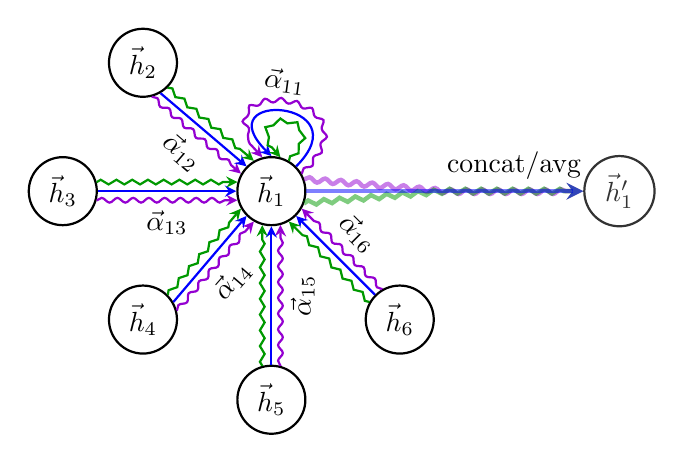
\begin{tikzpicture}

	\node[circle, draw, thick] (h1) {$\vec{h}_1$};
	\node[circle, draw, thick, above left=of h1] (h4) {$\vec{h}_2$};
	\node[circle, draw, thick, left=5em of h1] (h5) {$\vec{h}_3$};
	\node[circle, draw, thick, below left=of h1] (h6) {$\vec{h}_4$};
	\node[circle, draw, thick, below=5em of h1] (h7) {$\vec{h}_5$};
	\node[circle, draw, thick, below right=of h1] (h8) {$\vec{h}_6$};
	
	\draw[-stealth, mymauve, thick,decoration={snake, pre length=0.01mm, segment length=2mm, amplitude=0.3mm, post length=1.5mm}, decorate] (h8.120) -- node[sloped, above, black] {$\vec{\alpha}_{16}$} (h1.-30);
	\draw[-stealth, blue, thick] (h8.135) -- (h1.-45);
	\draw[-stealth, mygreen, thick, decoration={zigzag, pre length=0.01mm, segment length=2mm, amplitude=0.3mm, post length=1.5mm}, decorate] (h8.150) -- (h1.-60);
	
	\draw[-stealth, mymauve, thick,decoration={snake, pre length=0.01mm, segment length=2mm, amplitude=0.3mm, post length=1.5mm}, decorate] (h1.30) to[looseness=7] node[sloped, above, black] {$\vec{\alpha}_{11}$}(h1.105);
	\draw[-stealth, blue, thick] (h1.45) to[looseness=9] (h1.90);
	\draw[-stealth, mygreen, thick, decoration={zigzag, pre length=0.01mm, segment length=2mm, amplitude=0.3mm, post length=1.5mm}, decorate] (h1.60) to[looseness=20] (h1.75);
	
	\draw[-stealth, mymauve, thick,decoration={snake, pre length=0.01mm, segment length=2mm, amplitude=0.3mm, post length=1.5mm}, decorate] (h4.285) -- node[sloped, below, black] {$\vec{\alpha}_{12}$}(h1.150);
	\draw[-stealth, blue, thick] (h4.300) -- (h1.135);
	\draw[-stealth, mygreen, thick, decoration={zigzag, pre length=0.01mm, segment length=2mm, amplitude=0.3mm, post length=1.5mm}, decorate] (h4.315) -- (h1.120);
	
	\draw[-stealth, mymauve, thick,decoration={snake, pre length=0.01mm, segment length=2mm, amplitude=0.3mm, post length=1.5mm}, decorate] (h5.-15) -- node[sloped, below, black] {$\vec{\alpha}_{13}$}(h1.195);
	\draw[-stealth, blue, thick] (h5.0) -- (h1.180);
	\draw[-stealth, mygreen, thick, decoration={zigzag, pre length=0.01mm, segment length=2mm, amplitude=0.3mm, post length=1.5mm}, decorate] (h5.15) -- (h1.165);
	
		\draw[-stealth, mymauve, thick,decoration={snake, pre length=0.01mm, segment length=2mm, amplitude=0.3mm, post length=1.5mm}, decorate] (h6.15) -- node[sloped, below, black] {$\vec{\alpha}_{14}$}(h1.240);
	\draw[-stealth, blue, thick] (h6.30) -- (h1.225);
	\draw[-stealth, mygreen, thick, decoration={zigzag, pre length=0.01mm, segment length=2mm, amplitude=0.3mm, post length=1.5mm}, decorate] (h6.45) -- (h1.210);
	
	\draw[-stealth, mymauve, thick,decoration={snake, pre length=0.01mm, segment length=2mm, amplitude=0.3mm, post length=1.5mm}, decorate] (h7.75) -- node[sloped, below, black] {$\vec{\alpha}_{15}$}(h1.-75);
	\draw[-stealth, blue, thick] (h7.90) -- (h1.-90);
	\draw[-stealth, mygreen, thick, decoration={zigzag, pre length=0.01mm, segment length=2mm, amplitude=0.3mm, post length=1.5mm}, decorate] (h7.105) -- (h1.-105);
	
	\node[circle, draw, thick, right=10em of h1, opacity=0.8] (hp) {$\vec{h}_1'$};
	
	\coordinate[right=5em of h1] (A);
	
	\draw[-stealth,  mymauve, opacity=0.5, ultra thick,decoration={snake, pre length=0.01mm, segment length=2mm, amplitude=0.3mm, post length=1.5mm}, decorate] (h1.20) -- (A) -- (hp);
	\draw[-stealth, mygreen, opacity=0.5, ultra thick,decoration={zigzag, pre length=0.01mm, segment length=2mm, amplitude=0.3mm, post length=1.5mm}, decorate] (h1.-20) -- (A) -- (hp);
	\draw[-stealth, blue, opacity=0.5, ultra thick] (h1.0) -- (A) -- node[black, above, opacity=1.0] {concat/avg} (hp);

\end{tikzpicture}




\end{figure}

\end{frame}

\begin{frame}{Benefits of Spatial-based GNNs}
    \begin{itemize}
        \item Localized computation makes spatial GNNs efficient for large, dynamic graphs.
        \item No dependency on the global graph structure, unlike spectral methods.
        \item Attention mechanisms allow fine-tuned aggregation, useful for complex relational data.
        \item Applications in social networks, recommendation systems, and knowledge graphs.
    \end{itemize}
\end{frame}

\begin{frame}{Limitations of Spatial-based GNNs}
    \begin{itemize}
        \item Aggregation methods can oversimplify node information, leading to potential loss of unique node features.
        \item Spatial-based GNNs struggle with long-range dependencies due to limited neighborhood scope.
        \item May suffer from over-smoothing, where repeated aggregations make node representations indistinguishable.
        \item High memory and computation costs when aggregating large numbers of neighbors, especially for high-degree nodes.
        \item Lack of global context can limit performance on tasks requiring global structural information.
    \end{itemize}
\end{frame}

% % Materials and Methods
%   Datasets
%   MST
%   OPF

\section{Materials and Methods}

\begin{frame}{MILP Model - Graph Modelling}
    \begin{itemize}
        \item Proposal of a Mixed-Integer Linear Programming (MILP) model to solve the problem.
        \item Graph construction representing spatio-temporal permits shared by the drones.
        \item Modeled as a directed graph (digraph) $G = (V, A)$.
        \item $V$: set of nodes representing airspace and virtual drone locations.
        \item $A$: set of directed arcs representing permitted transitions between nodes.
    \end{itemize}
\end{frame}


\begin{frame}{MILP Model - Virtual Nodes}
    \begin{figure}
      \begin{columns}
        \column{.4\linewidth}
        \begin{itemize}
           
            \item Source node $b_k$: Starting point of drone $k$'s mission.
            \item Sink node $e_k$: Ending point of drone $k$'s mission.
            
            \item Focus on spatial topology, omitting temporal component.
        \end{itemize}
        \caption{Graph modelling. \\ Source: The authors.}
        \label{fig_graph}
        \column{.45\linewidth}
        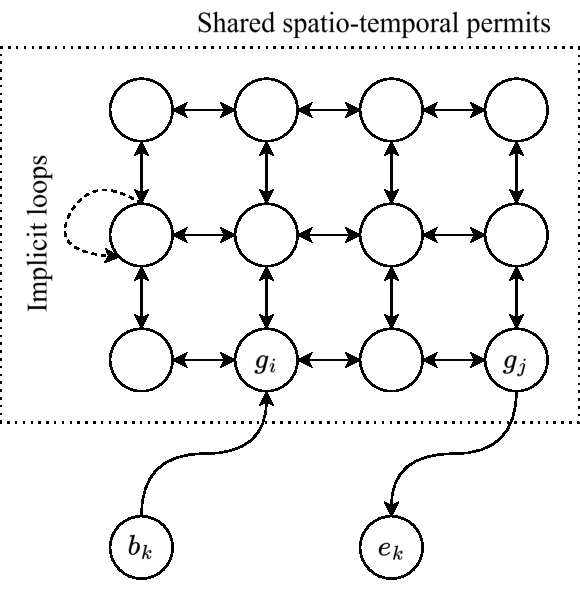
\includegraphics[width=0.8\textwidth]{img/graph_model.pdf}
      \end{columns}
    \end{figure}
\end{frame}


\begin{frame}{MILP Model - Parameters}
    \begin{itemize}
        \item $T$: Maximum time allowed for the mission.
        \item $b_k$: Initial virtual vertex representing the initial position of drone $k$.
        \item $e_k$: Final virtual vertex representing the final position of drone $k$.
        \item $\mathcal{R}$: Set of drones.
        \item $\mathcal{G}$: Digraph $(\mathcal{V}, \mathcal{A})$ representing the airspace.
        \item $\mathcal{V}$: Set of vertices of $\mathcal{G}$.
        \item $\mathcal{B} \subset \mathcal{V}$: Set of initial virtual vertices $b_k$.
        \item $\mathcal{E} \subset \mathcal{V}$: Set of final virtual vertices $e_k$.
        \item $\mathcal{S}$: Set $\mathcal{V} \setminus (\mathcal{B} \cup \mathcal{E})$.
        \item $\mathcal{A}$: Set of arcs $(i,j) \in \mathcal{A}$ of $\mathcal{G}$.
    \end{itemize}
\end{frame}

\begin{frame}{MILP Model - Variables}
    \begin{itemize}
        \item Decision Variables:
        \begin{itemize}
            \item $x_{i,j,t}^k = 1 \iff$ drone $k$ jumps from $i$ to $j$ at time $t$.
        \end{itemize}
        \item Indices:
        \begin{itemize}
            \item $k$: Drone $\implies k \in \mathcal{R}$.
            \item $t$: Time $\implies 1 \leq t \leq T$.
            \item $i, j, l$: Vertices $\implies i, j, l \in \mathcal{V}$.
        \end{itemize}
    \end{itemize}
\end{frame}


\begin{frame}{MILP Model - Objective Function}
    \begin{itemize}
        \item Minimize the total sum of the number of drone movements:
    \end{itemize}
    \[
    \min
    \sum_{k \in \mathcal{R}}
    \sum_{t=1}^T
    \sum_{ \; (i,j) \in \mathcal{A}:\ j \notin (\mathcal{E} \cup \mathcal{B})} x_{i,j,t}^{k}
    \]
    \begin{itemize}
        \item Minimize the total number of drone movements, counting $n-1$ jumps for each drone that performs $n$ jumps.
    \end{itemize}
\end{frame}

\begin{frame}{MILP Model - Constraints}
    \begin{itemize}
        \item Ensure each drone starts its mission:
    \end{itemize}
    \[
    \sum_{t=1}^{T}
    \sum_{j \in \mathcal{S}}
    x_{b_k,j,t}^k = 1, \quad \forall k \in \mathcal{R}
    \]
    \begin{itemize}
        \item Flow conservation:
    \end{itemize}
    \[
    \sum_{j \in \mathcal{V}} x_{i,j,t-1}^{k} =
    \sum_{l \in \mathcal{V}} x_{j,l,t}^{k}, \quad
    \forall j \in \mathcal{V}, \forall k \in \mathcal{R}, \forall t \in \{2, \ldots, T\}
    \]
\end{frame}

\begin{frame}{MILP Model - Constraints (Cont.)}
    \begin{itemize}
        \item Border condition at time $t=0$:
    \end{itemize}
    \[
    x_{i,j,0}^k = \left\{
    \begin{matrix}
        1, & \text{if}\ i=b_k \land j=b_k,\\
        0, & \text{otherwise}.
    \end{matrix}
    \right.
    \quad \forall k \in \mathcal{R}, \forall (i,j) \in A
    \]
    \begin{itemize}
        \item Mutual exclusion of vertex occupation:
    \end{itemize}
    \[
    \sum_{k \in \mathcal{R}}
    \sum_{j \in \mathcal{V}}
    x_{i,j,t}^{k} \leq 1, \quad \forall j \in \mathcal{V}, \forall t \in \{1, \ldots, T\}
    \]
\end{frame}

\begin{frame}{MILP Model - Mission Accomplishment}
    \begin{itemize}
        \item Ensure each drone completes its mission:
    \end{itemize}
    \[
    \sum_{t=1}^{T}
    \sum_{i \in \mathcal{S}}
    x_{i,e_k,t}^k \geq 1, \quad \forall k \in \mathcal{R}
    \]
\end{frame}

\begin{frame}{Heuristic Approach}
        \begin{itemize}
            \item Utilize distance measure as heuristic metric \cite{Weise2023}.
            \item Organize drones in ascending order (prioritized planning) based on start and end points.
            \item Employ iterative Breadth-First Search (BFS) on temporal graph.
            \item Dynamic constraints update of occupied positions (conflict-based search).
            \item Combine heuristic sorting and iterative BFS for efficient path planning and adaptability.
        \end{itemize}
\end{frame}


\begin{frame}{Algorithm Notation}
    \begin{table}
      \centering
      \caption{Notation used in the Algorithm.}
      \label{tab:notation}
      \begin{tabular}{ll}
        \toprule
        Notation & Definition \\
        \midrule
        $\mathcal{V}$ &Set of vertices in the graph $: (i,j,t)$ \\
        $\mathcal{E}$ & Set of edges  \\
        $\mathcal{D}$ & Set of drones \\
        $\mathcal{S}$ & Set of already scheduled vertices \\
        $\mathcal{P}_d \subseteq \mathcal{V} $ & Path of drone $d$ \\
        $\mathcal{G} = (\mathcal{V},\mathcal{E}) $ & Temporal Graph \\
        \bottomrule
      \end{tabular}
    \end{table}
\end{frame}

\begin{frame}{Heuristic Algorithm Steps}
    \begin{enumerate}
        \item \textbf{Drones Sorting}: Ascending sort using Euclidean Distance.
            \begin{equation}
                \mathcal{D}_{\text{sorted}} = \text{sort}(\mathcal{D}, \text{heuristic})
            \end{equation}
        \item \textbf{Path for Each Drone}: Compute path \(P_d\) using BFS on graph \(\mathcal{G}\).
            \begin{equation}
                \forall d \in \mathcal{D}_{\text{sorted}}: \quad \mathcal{P}_d = \text{BFS}(\mathcal{G}, d)
            \end{equation}
        \item \textbf{Constraints Update}: Update set of already scheduled vertices \(\mathcal{S}\).
            \begin{equation}
                \mathcal{S} = \mathcal{S} \cup \bigcup_{d \in \mathcal{D}_{\text{sorted}}} \mathcal{P}_d
            \end{equation}
    \end{enumerate}
\end{frame}

\begin{frame}{Algorithm Visualization}
    \begin{figure}[h]
    \centering
    \begin{tikzpicture}[scale=.8, every node/.style={minimum size=1cm}]

        % Define quadcopter style
        \tikzset{
            quadcopter/.style={
                quadcopter side,
                fill=white,
                draw=gray,
                minimum width=1cm,
                below=of second-scope, 
            },
        }
        
        % Add another drone
        \node (quadcopterGreen) [quadcopter side, fill=white, draw=greenMW, minimum width=1cm, rotate=0] at (5,1) {};

        \node (quadcopterBrown) [quadcopter side, fill=white, draw=brown, minimum width=1cm, rotate=0] at (5,-11.3) {};

        \node (quadcopterOrange) [quadcopter side, fill=white, draw=orange, minimum width=1cm, rotate=0] at (4.4,-14.3) {};

        \node (quadcopterBlue) [quadcopter side, fill=white, draw=blue, minimum width=1cm, rotate=0] at (-5,-8.2) {};
        
        % Último Escopo (t=6)
        \begin{scope}[yshift=-423, every node/.append style={yslant=0.5, xslant=-1}, yslant=0.5, xslant=-1]

            

            \fill[white, fill opacity=0.9] (0,0) rectangle (5,5);
            
            \draw[step=4mm, black] (0,0) grid (5,5);
            \draw[black, thick] (0,0) rectangle (5,5); % Borders
            \fill[orange] (2.05,2.05) rectangle (2.35,2.35); % center pixel
            \node (centerBegint2) at (2.2,2.2) {B}; % place 'B' in the center
            % \fill[greenMW] (1.65,2.05) rectangle (1.95,2.35); % left
            % \fill[greenMW] (2.45,2.05) rectangle (2.75,2.35); % right
            \fill[orange] (2.05,1.95) rectangle (2.35,1.65); % bottom
            \fill[orange,yshift=-11.2] (2.05,1.95) rectangle (2.35,1.65); % bottom
            \fill[orange,yshift=-22.5] (2.05,1.95) rectangle (2.35,1.65); % bottom
            \fill[orange,yshift=-33.5] (2.05,1.95) rectangle (2.35,1.65); % bottom
            
            %\fill[greenMW] (2.05,2.45) rectangle (2.35,2.75); % top
            % 8 -pixel setting
           
            % \fill[greenMW] (2.75,1.95) rectangle (2.45,1.65); % bottom-right
            % \fill[greenMW] (1.65,1.95) rectangle (1.95,1.65); % bottom-left
            
            \node (landedOrange) at (1.5,0.8) {};

            \node(pathdestinyt6) [black, font=\bfseries] at ([yshift=-45.3]centerBegint2) {E};
        \end{scope}



        % Penúltimo Escopo (t=5)
        \begin{scope}[yshift=-340, every node/.append style={yslant=0.5, xslant=-1}, yslant=0.5, xslant=-1]
            \fill[white, fill] (0,0) rectangle (5,5);
            \draw[step=4mm, black] (0,0) grid (5,5);
            \draw[black, thick] (0,0) rectangle (5,5); % Borders
            \fill[orange!55] (2.05,2.05) rectangle (2.35,2.35); % center pixel
            \node (centerBegint3) at (2.2,2.2) {B}; % place 'B' in the center

            \fill[orange!55,xshift=-22.6] (2.45,2.05) rectangle (2.75,2.35); % most left
            

            \node (landedBrown) at (1.5,0.6) {};

            %\fill[blue] (1.65,2.05) rectangle (1.95,2.35); % left
            % left X
            \draw[orange] (1.65,2.05) -- (1.95,2.35);
            \draw[orange] (1.65,2.35) -- (1.95,2.05);
            % left bottom X
            \draw[orange, yshift=-11.3] (1.65,2.05) -- (1.95,2.35);
            \draw[orange, yshift=-11.3] (1.65,2.35) -- (1.95,2.05);   
            % most left X
            \draw[orange, xshift=-11.3] (1.65,2.05) -- (1.95,2.35);
            \draw[orange, xshift= -11.3] (1.65,2.35) -- (1.95,2.05);   

            \fill[orange!55,xshift=11.3] (2.45,2.05) rectangle (2.75,2.35); % most right
            % most right X
            \draw[orange, xshift=34.4] (1.65,2.05) -- (1.95,2.35);
            \draw[orange, xshift=34.4] (1.65,2.35) -- (1.95,2.05);

            % bottom center right X
            \draw[orange, xshift=34.4, yshift= -11.3] (1.65,2.05) -- (1.95,2.35);
            \draw[orange, xshift=34.4, yshift= -11.3] (1.65,2.35) -- (1.95,2.05);

            %  top center right X
            \draw[orange, xshift=34.4, yshift= 11.3] (1.65,2.05) -- (1.95,2.35);
            \draw[orange, xshift=34.4, yshift= 11.3] (1.65,2.35) -- (1.95,2.05);
            
            % most most right X
            \draw[orange, xshift=34.4 + 11.3] (1.65,2.05) -- (1.95,2.35);
            \draw[orange, xshift=34.4 + 11.3] (1.65,2.35) -- (1.95,2.05);

            

            \fill[orange!55] (2.45,2.05) rectangle (2.75,2.35); % right
            
            \fill[orange!55] (2.05,2.45) rectangle (2.35,2.75); % top
            \fill[orange!55, xshift=11.3] (2.05,2.45) rectangle (2.35,2.75); % top right
            \fill[orange!55, xshift=-11.3] (2.05,2.45) rectangle (2.35,2.75); % top left
            \fill[orange!55, yshift=11.3] (2.05,2.45) rectangle (2.35,2.75); % most top
            \fill[orange!55] (2.05,1.95) rectangle (2.35,1.65); % bottom

            \fill[orange!55, xshift= 11.3] (2.05,1.95) rectangle (2.35,1.65); % bottom right

            \fill[orange!55,yshift=-11.3] (2.05,1.95) rectangle (2.35,1.65); % most bottom
            
            %\fill[greenMW] (1.65,2.45) rectangle (1.95,2.75); % top-left 
            % top left X
            \draw[orange] (1.65,2.75) -- (1.95,2.45);
            \draw[orange] (1.65,2.45) -- (1.95,2.75);
            
            % top most left X
            \draw[orange, xshift=-11.3] (1.65,2.75) -- (1.95,2.45);
            \draw[orange, xshift=-11.3] (1.65,2.45) -- (1.95,2.75);
            
            % \draw[orange,xshift=-11.3] (1.65,2.75) -- (1.95,2.45);
            % \draw[orange,xshift=-11.3] (1.65,2.45) -- (1.95,2.75);   

            %\fill[greenMW] (2.45,2.45) rectangle (2.75,2.75); % top-right
            \draw[orange] (2.45,2.45) -- (2.75,2.75);
            \draw[orange] (2.45,2.75) -- (2.75,2.45);

            %\fill[greenMW] (2.75,1.95) rectangle (2.45,1.65); % bottom-right
            \draw[orange] (2.45,1.95) -- (2.75,1.65);
            \draw[orange] (2.45,1.65) -- (2.75,1.95);

            % top most X 
            \draw[orange,xshift= -34 +45.4,yshift=11] (1.65,2.75) -- (1.95,2.45);
            \draw[orange,xshift=-34 +45.4,yshift=11] (1.65,2.45) -- (1.95,2.75);

            % top most right X 
            \draw[orange,xshift= -34 +45.4 + 11.2,yshift=11] (1.65,2.75) -- (1.95,2.45);
            \draw[orange,xshift=-34 +45.4 + 11.2,yshift=11] (1.65,2.45) -- (1.95,2.75);

            % top most left X 
            \draw[orange,xshift= -34 +45.4 - 11.2,yshift=11] (1.65,2.75) -- (1.95,2.45);
            \draw[orange,xshift=-34 +45.4 - 11.2,yshift=11] (1.65,2.45) -- (1.95,2.75);

            % top most last X 
            \draw[orange,xshift= -34 +45.4 ,yshift=22.2] (1.65,2.75) -- (1.95,2.45);
            \draw[orange,xshift=-34 +45.4 ,yshift=22.2] (1.65,2.45) -- (1.95,2.75);

            % bottom most X
            \draw[orange,xshift= -34 +45.4,yshift=-34.4] (1.65,2.75) -- (1.95,2.45);
            \draw[orange,xshift=-34 +45.4,yshift=-34.4] (1.65,2.45) -- (1.95,2.75);

            % bottom most right X
            \draw[orange,xshift= -34 +45.4 +11.2 ,yshift=-34.4] (1.65,2.75) -- (1.95,2.45);
            \draw[orange,xshift=-34 +45.4 + 11.2,yshift=-34.4] (1.65,2.45) -- (1.95,2.75);

            % bottom most left X
            \draw[orange,xshift= -34 +45.4 -11.2 ,yshift=-34.4] (1.65,2.75) -- (1.95,2.45);
            \draw[orange,xshift=-34 +45.4  -11.2,yshift=-34.4] (1.65,2.45) -- (1.95,2.75);

            % bottom most last X
            \draw[orange,xshift= -34 +45.4,yshift=-45.8] (1.65,2.75) -- (1.95,2.45);
            \draw[orange,xshift=-34 +45.4,yshift=-45.8] (1.65,2.45) -- (1.95,2.75);

                    

            %\fill[blue] (1.65,1.95) rectangle (1.95,1.65); % bottom-left
            % 2. ring
            %\fill[greenMW] (1.25,1.55) rectangle (1.55,1.25); % bottom-left
            %\fill[greenMW] (0.85,1.55) rectangle (1.15,1.25); % bottom-left
            %\fill[greenMW] (0.85,1.15) rectangle (1.15,0.85); % bottom-left

            \fill[brown, xshift=22.7, yshift=-11.2] (1.25,0.75) rectangle (1.55,0.45); % bottom-left

            \node(pathdestinyt3) [black, font=\bfseries] at ([yshift=-45.3]centerBegint3) {E};
        \end{scope}


        % Escopo (t=4)
        \begin{scope}[yshift=-250, every node/.append style={yslant=0.5, xslant=-1}, yslant=0.5, xslant=-1]
            \fill[white, fill] (0,0) rectangle (5,5);
            \draw[step=4mm, black] (0,0) grid (5,5);
            \draw[black, thick] (0,0) rectangle (5,5); % Borders
            \fill[orange!55] (2.05,2.05) rectangle (2.35,2.35); % center pixel
            \node (centerBegint3) at (2.2,2.2) {B}; % place 'B' in the center
            
            %\fill[blue] (1.65,2.05) rectangle (1.95,2.35); % left
            \draw[orange] (1.65,2.05) -- (1.95,2.35);
            \draw[orange] (1.65,2.35) -- (1.95,2.05);   

            \node (landedBlue) at (1.1,2.3) {};

            % most right X
            \draw[orange, xshift=34.4] (1.65,2.05) -- (1.95,2.35);
            \draw[orange, xshift=34.4] (1.65,2.35) -- (1.95,2.05);  

            \fill[orange!55] (2.45,2.05) rectangle (2.75,2.35); % right
            \fill[orange!55] (2.05,2.45) rectangle (2.35,2.75); % top
            \fill[orange!55] (2.05,1.95) rectangle (2.35,1.65); % bottom
            
            %\fill[greenMW] (1.65,2.45) rectangle (1.95,2.75); % top-left
            \draw[orange] (1.65,2.75) -- (1.95,2.45);
            \draw[orange] (1.65,2.45) -- (1.95,2.75);   
            
            % \draw[orange,xshift=-11.3] (1.65,2.75) -- (1.95,2.45);
            % \draw[orange,xshift=-11.3] (1.65,2.45) -- (1.95,2.75);   

            %\fill[greenMW] (2.45,2.45) rectangle (2.75,2.75); % top-right
            \draw[orange] (2.45,2.45) -- (2.75,2.75);
            \draw[orange] (2.45,2.75) -- (2.75,2.45);

            %\fill[greenMW] (2.75,1.95) rectangle (2.45,1.65); % bottom-right
            \draw[orange] (2.45,1.95) -- (2.75,1.65);
            \draw[orange] (2.45,1.65) -- (2.75,1.95);

            % top most X 
            \draw[orange,xshift= -34 +45.4,yshift=11] (1.65,2.75) -- (1.95,2.45);
            \draw[orange,xshift=-34 +45.4,yshift=11] (1.65,2.45) -- (1.95,2.75);

            % bottom most X
            \draw[orange,xshift= -34 +45.4,yshift=-34.4] (1.65,2.75) -- (1.95,2.45);
            \draw[orange,xshift=-34 +45.4,yshift=-34.4] (1.65,2.45) -- (1.95,2.75);

            \fill[blue] (1.65,1.95) rectangle (1.95,1.65); % bottom-left
            % 2. ring
            %\fill[greenMW] (1.25,1.55) rectangle (1.55,1.25); % bottom-left
            %\fill[greenMW] (0.85,1.55) rectangle (1.15,1.25); % bottom-left
            %\fill[greenMW] (0.85,1.15) rectangle (1.15,0.85); % bottom-left

            \fill[brown, xshift=22.6] (1.25,0.75) rectangle (1.55,0.45); % bottom-left

            \node(pathdestinyt3) [black, font=\bfseries] at ([yshift=-45.3]centerBegint3) {E};
        \end{scope}

        % Terceiro Escopo (t=3)
        \begin{scope}[yshift=-166, every node/.append style={yslant=0.5, xslant=-1}, yslant=0.5, xslant=-1]
            \fill[white, fill opacity=0.9] (0,0) rectangle (5,5);
            \draw[step=4mm, black] (0,0) grid (5,5);
            \draw[black, thick] (0,0) rectangle (5,5); % Borders
            \fill[orange!55] (2.05,2.05) rectangle (2.35,2.35); % lighter orange for center pixel
            \node (centerBegint3) at (2.2,2.2) {B}; % place 'B' in the center
            \fill[blue] (1.65,2.05) rectangle (1.95,2.35); % left
            \draw[orange] (2.45,2.05) -- (2.75,2.35);
            \draw[orange] (2.45,2.35) -- (2.75,2.05);
            %\fill[greenMW] (2.05,2.45) rectangle (2.35,2.75); % top
            \draw[orange] (2.05,2.45) -- (2.35,2.75);
            \draw[orange] (2.05,2.75) -- (2.35,2.45);

            %\fill[greenMW] (2.05,1.95) rectangle (2.35,1.65); % bottom
            \draw[orange] (2.05,1.95) -- (2.35,1.65);
            \draw[orange] (2.05,1.65) -- (2.35,1.95);

            
            %\fill[greenMW] (1.65,2.45) rectangle (1.95,2.75); % top-left
            %\fill[greenMW] (2.45,2.45) rectangle (2.75,2.75); % top-right
            %\fill[greenMW] (2.75,1.95) rectangle (2.45,1.65); % bottom-right
            %\fill[greenMW] (1.65,1.95) rectangle (1.95,1.65); % bottom-left
            % 2. ring
            %\fill[greenMW] (1.25,1.55) rectangle (1.55,1.25); % bottom-left
            %\fill[greenMW] (0.85,1.55) rectangle (1.15,1.25); % bottom-left
            %\fill[greenMW] (0.85,1.15) rectangle (1.15,0.85); % bottom-left

            \fill[brown, xshift=11.3] (1.25,0.75) rectangle (1.55,0.45); % bottom-left

            \node(pathdestinyt3) [black, font=\bfseries] at ([yshift=-45.3]centerBegint3) {E};

            \node(midpointX) at (2.6, 2.2){};
            
        \end{scope}

        % Escopo do meio (t=2)
        \begin{scope}[yshift=-83, every node/.append style={yslant=0.5, xslant=-1}, yslant=0.5, xslant=-1]

            \node [quadcopter side,fill=white,draw=orange,minimum width=1cm,rotate=10] (quadcoptert2) at (1,7) {};

            \fill[white, fill opacity=0.9] (0,0) rectangle (5,5);

            \node (arrivalOrange) at (1.8,2.1) {};
            
            \draw[step=4mm, black] (0,0) grid (5,5);
            \draw[black, thick] (0,0) rectangle (5,5); % Borders
            \fill[orange] (2.05,2.05) rectangle (2.35,2.35); % center pixel
            \node (centerBegint2) at (2.2,2.2) {B}; % place 'B' in the center
            % \fill[greenMW] (1.65,2.05) rectangle (1.95,2.35); % left
            % \fill[greenMW] (2.45,2.05) rectangle (2.75,2.35); % right
            \fill[greenMW] (2.05,1.95) rectangle (2.35,1.65); % bottom
            \node (landedGreen) at (1.8,1.9) {};
            %\fill[greenMW] (2.05,2.45) rectangle (2.35,2.75); % top
            % 8 -pixel setting
            \fill[blue] (1.65,2.45) rectangle (1.95,2.75); % top-left
            % \fill[greenMW] (2.45,2.45) rectangle (2.75,2.75); % top-right
            % \fill[greenMW] (2.75,1.95) rectangle (2.45,1.65); % bottom-right
            % \fill[greenMW] (1.65,1.95) rectangle (1.95,1.65); % bottom-left
            % 2. ring
            % \fill[greenMW] (1.25,1.55) rectangle (1.55,1.25); % bottom-left
            % \fill[greenMW] (0.85,1.55) rectangle (1.15,1.25); % bottom-left
            % \fill[greenMW] (0.85,1.15) rectangle (1.15,0.85); % bottom-left
            \fill[brown] (1.25,0.75) rectangle (1.55,0.45); % bottom-left
            \node(pathdestinyt2) [black, font=\bfseries] at ([yshift=-45.3]centerBegint2) {E};
        \end{scope}

        % Primeiro Escopo (t=1)
        \begin{scope}[yshift=0, every node/.append style={yslant=0.5, xslant=-1}, yslant=0.5, xslant=-1]

           \node [quadcopter side,fill=white,draw=orange,minimum width=1cm,rotate=10] (quadcoptert1) at (3,7.6) {};
            
           \node (orangeTakeOff) at (2.5,1.8) {};
        
            \fill[white, fill opacity=0.9] (0,0) rectangle (5,5);
            \draw[step=4mm, black] (0,0) grid (5,5); % Grid definition
            \draw[black, thick] (0,0) rectangle (5,5); % Borders
            \fill[greenMW] (2.05,2.05) rectangle (2.35,2.35); % center pixel
            \draw[red, thin] (2.05,2.05) rectangle (2.35,2.35); % border
            \node (centerBegint1) at (2.2,2.2) {B}; % place 'B' in the center
            \fill[blue] (2.05,2.45) rectangle (2.35,2.75); % top
            % \fill[blue] (1.65,2.45) rectangle (1.95,2.75); % top-left
            % \fill[blue] (2.45,2.45) rectangle (2.75,2.75); % top-right
            % \fill[blue] (2.75,1.95) rectangle (2.45,1.65); % bottom-right
            % \fill[blue] (1.65,1.95) rectangle (1.95,1.65); % bottom-left
            % % 2. ring
            % \fill[blue] (1.25,1.55) rectangle (1.55,1.25); % bottom-left
            % \fill[blue] (0.85,1.55) rectangle (1.15,1.25); % bottom-left
            % \fill[blue] (0.85,1.15) rectangle (1.15,0.85); % bottom-left
            % \fill[blue] (1.25,0.75) rectangle (1.55,0.45); % bottom-left

            \fill[brown, xshift= -11.3] (1.25,0.75) rectangle (1.55,0.45); % bottom-left
            
            % Insert 'E' three squares down the center
            \node(pathdestinyt1) [black, font=\bfseries] at ([yshift=-45.3]centerBegint1) {E};
            
        \end{scope}

        % Draw annotations
        \draw[-latex, thick, gray, dashed] (-5.4,-3.5) node[left] {occupied} to[out=0, in=200] (-0.5,-4.1);

        \draw[-latex, thick, red] (quadcoptert1) to[out=35, in=90] node[midway, above] {failed takeoff} (orangeTakeOff);

        \draw[-latex, thick, orange] (quadcoptert2) to[out=0, in=10] node[very near start, above] {arrival} (arrivalOrange);

        %\draw[-latex, thick, orange] ([xshift=-10]centerBegint3) to[out=0, in=10] (midpointX);

        \draw[thick, green!60!black, dashed] (landedGreen) to[out=0, in=10] node[above, pos=0.45 , font=\footnotesize] {landed} (quadcopterGreen);

        \draw[thick, brown!, dashed] (landedBrown) to[out=0, in=10] node[ above, pos=1 , font=\footnotesize] {landed} (quadcopterBrown);

        \draw[thick, orange!, dashed] (landedOrange) to[out=0, in=10] node[ above, pos=0.75 , font=\footnotesize] {path found} (quadcopterOrange);

        \draw[thick, blue!60!white, dashed] (landedBlue) to[out=0, in=13] node[ above, pos=0.85 , font=\footnotesize] {landed} (quadcopterBlue);

        % Annotations
        \draw[thick, gray!60!black] (6,4) node {t=1};
        \draw[thick, gray!60!black] (6,0) node {t=2};
        \draw[thick, gray!60!black] (6,-3) node {t=3};
        \draw[thick, gray!60!black] (6,-6) node {t=4};
        \draw[thick, gray!60!black] (6,-9) node {t=5};
        \draw[thick, gray!60!black] (6.2,-12.4) node {t=6};
    \end{tikzpicture}
    \caption{Algorithm visualization. Source: The authors.}
    \label{fig:visualgo}
\end{figure}

\end{frame}

\begin{frame}{Complexity Analysis and Boundedness}
    \begin{itemize}
        \item Worst-case complexity: $\mathcal{O}((N+M) K N M \log((N+M) K N M))$.
        \item Approximation: $\mathcal{O}(N^3 K \log(N^3 K))$ for square grids.
    \end{itemize}
    \begin{figure}
      \centering
      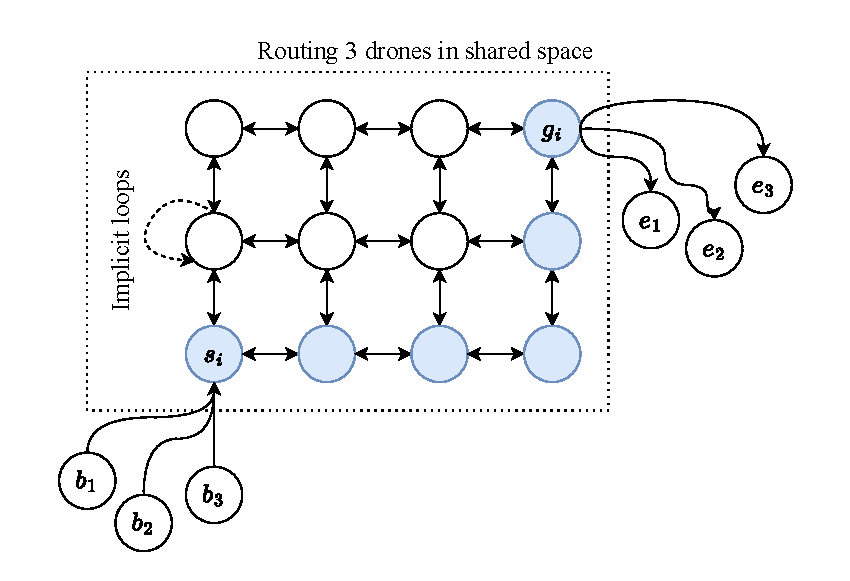
\includegraphics[width=0.6\textwidth]{img/worst_path.drawio.pdf}
      \caption{Worst case path. Source: The authors.}
      \label{fig:worst_path}
    \end{figure}
\end{frame}

\begin{frame}{Hybrid Methodology}
    \begin{itemize}
        \item \textbf{Heuristic Solution Generation}
            \begin{itemize}
                \item Quickly generates an initial feasible solution.
                \item Determines a plausible time horizon $T_{\text{heuristic}}$.
            \end{itemize}
        \item \textbf{MILP Model Refinement}
            \begin{itemize}
                \item Uses $T_{\text{heuristic}}$ and initial feasible solution from heuristic.
                \item Refines the solution to ensure global optimality.
            \end{itemize}
        \item \textbf{Advantages}
            \begin{itemize}
                \item Combines computational speed with solution accuracy.
                \item Skips multiple iterations to determine $T$, reducing computational expense.
            \end{itemize}
    \end{itemize}
\end{frame}




% %   Results
%   Difficulties, limitations, and future works

\section{Results}

\begin{frame}{Results}

    \begin{figure}[H]
    \centering
    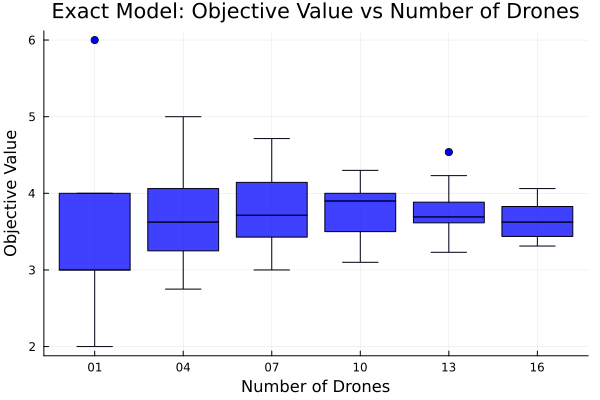
\includegraphics[width=0.57\textwidth]{img/julia_obj_boxplot_vs_drones.png}
    \caption{Exact Model Objective. Source: The authors.}
    \label{fig:exact_model_obj}
\end{figure}

\end{frame}

\begin{frame}{Results}

    \begin{figure}[H]
    \centering
    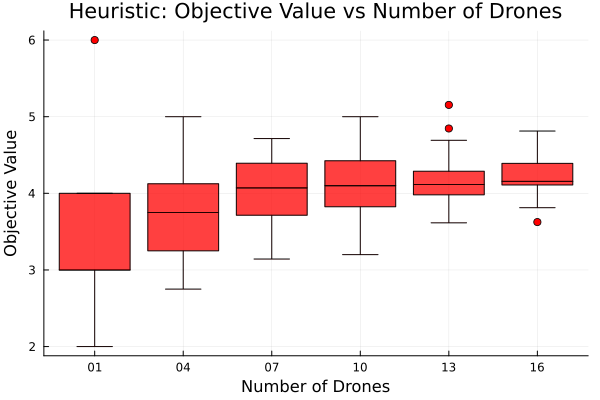
\includegraphics[width=0.57\textwidth]{img/cpp_obj_boxplot_vs_drones.png}
    \caption{Heuristic Objective. Source: The authors.}
    \label{fig:exact_model_obj}
\end{figure}

\end{frame}

\begin{frame}{Results}

\begin{figure}[H]
    \centering
    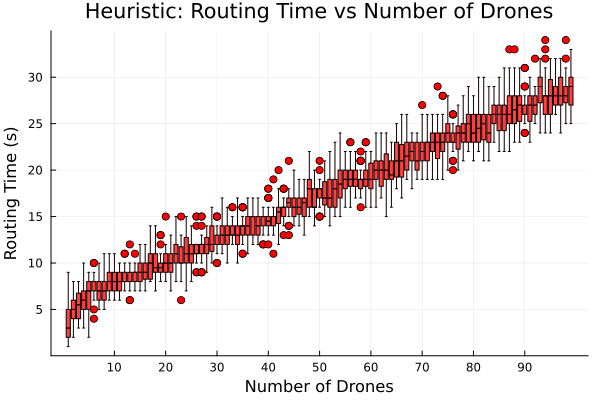
\includegraphics[width=0.57\textwidth]{img/cpp_routing_time_boxplot_vs_drones.png}
    \caption{Heuristic Routing Time ($T$) corresponding to Figure \ref{fig:heuristic_normalized_dist}. Source: The authors.}
    \label{fig:heuristic_normalized_routing_time}
\end{figure}


\end{frame}

% \begin{frame}{Results}



% \begin{figure}
%     \centering
%     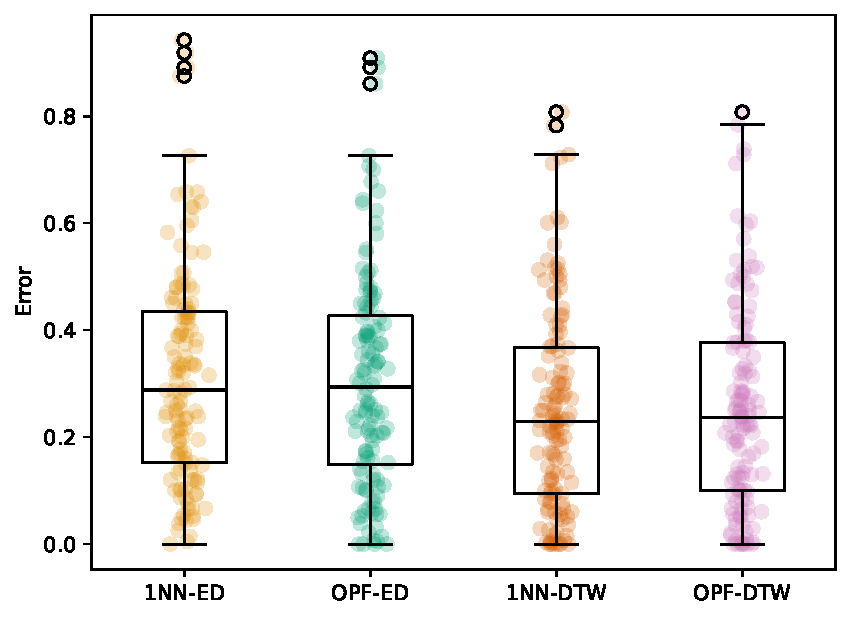
\includegraphics[width=0.5\linewidth]{img/boxplot.pdf}
%     \caption{Boxplot of classification errors for each classifier algorithm. Source: The authors.}
% \end{figure}

% \end{frame}

% \begin{frame}{Results}

% \begin{table}[!htbp]

% \begin{tabular}{ccccc}
% Algorithm & Mean &  Stdev & Wins/Draws/Losses & Wins/Draws/Losses \\
% & ($\mu$) & ($\sigma$) & against 1NN-ED & against 1NN-DTW\\
% \midrule
% OPF-ED & 0.30 & 0.20 & 37/25/66 & 35/7/86\\
% OPF-DTW & 0.25 & 0.19 & 85/7/36 & 14/36/78\\
% 1NN-ED & 0.31 & 0.20 & 0/128/0 & 38/4/86\\
% 1NN-DTW & 0.25 & 0.19 & 86/4/38 & 0/128/0\\
% \end{tabular}%
	
% 	\caption{Mean and standard variation of classification errors for each algorithm, and also the number of times they achieved a better, equal, and worst error than 1NN-ED and 1NN-DTW. Source: The authors.}%
% 	\label{tab:describe_errors} 
% \end{table}

% \end{frame}




\section{Conclusion and Future Works}

\begin{frame}{Conclusion}

\destaq{Advancements}

\begin{itemize}
    \item  Addressing the Last Mile Delivery Drones problem through a MAPF approach ;
    \item Ensuring collision avoidance and efficient airspace control.
    \item Significant advancement over previous algorithms with guaranteed finite and bounded polynomial time convergence for the heuristic
\end{itemize}

\bigskip

\destaq{Limitations}

\begin{itemize}
    \item Does not address real world problems like energy, fuel and speed of the drones;
    \item The experiment using binary search to find the T for the MILP in $\mathcal{O}( \log( T)$) is not conducted;
    \item Small grid sizes in experiments;
\end{itemize}

\end{frame}

\begin{frame}{Future Works}
    \begin{figure}
      \begin{columns}
        \column{.23\linewidth}
        \caption{Tradable Permit Model in the Decentralized LMDD. \\ Source: \cite{Verri}}
        \label{fig:trad_drones}
        \column{.75\linewidth}
        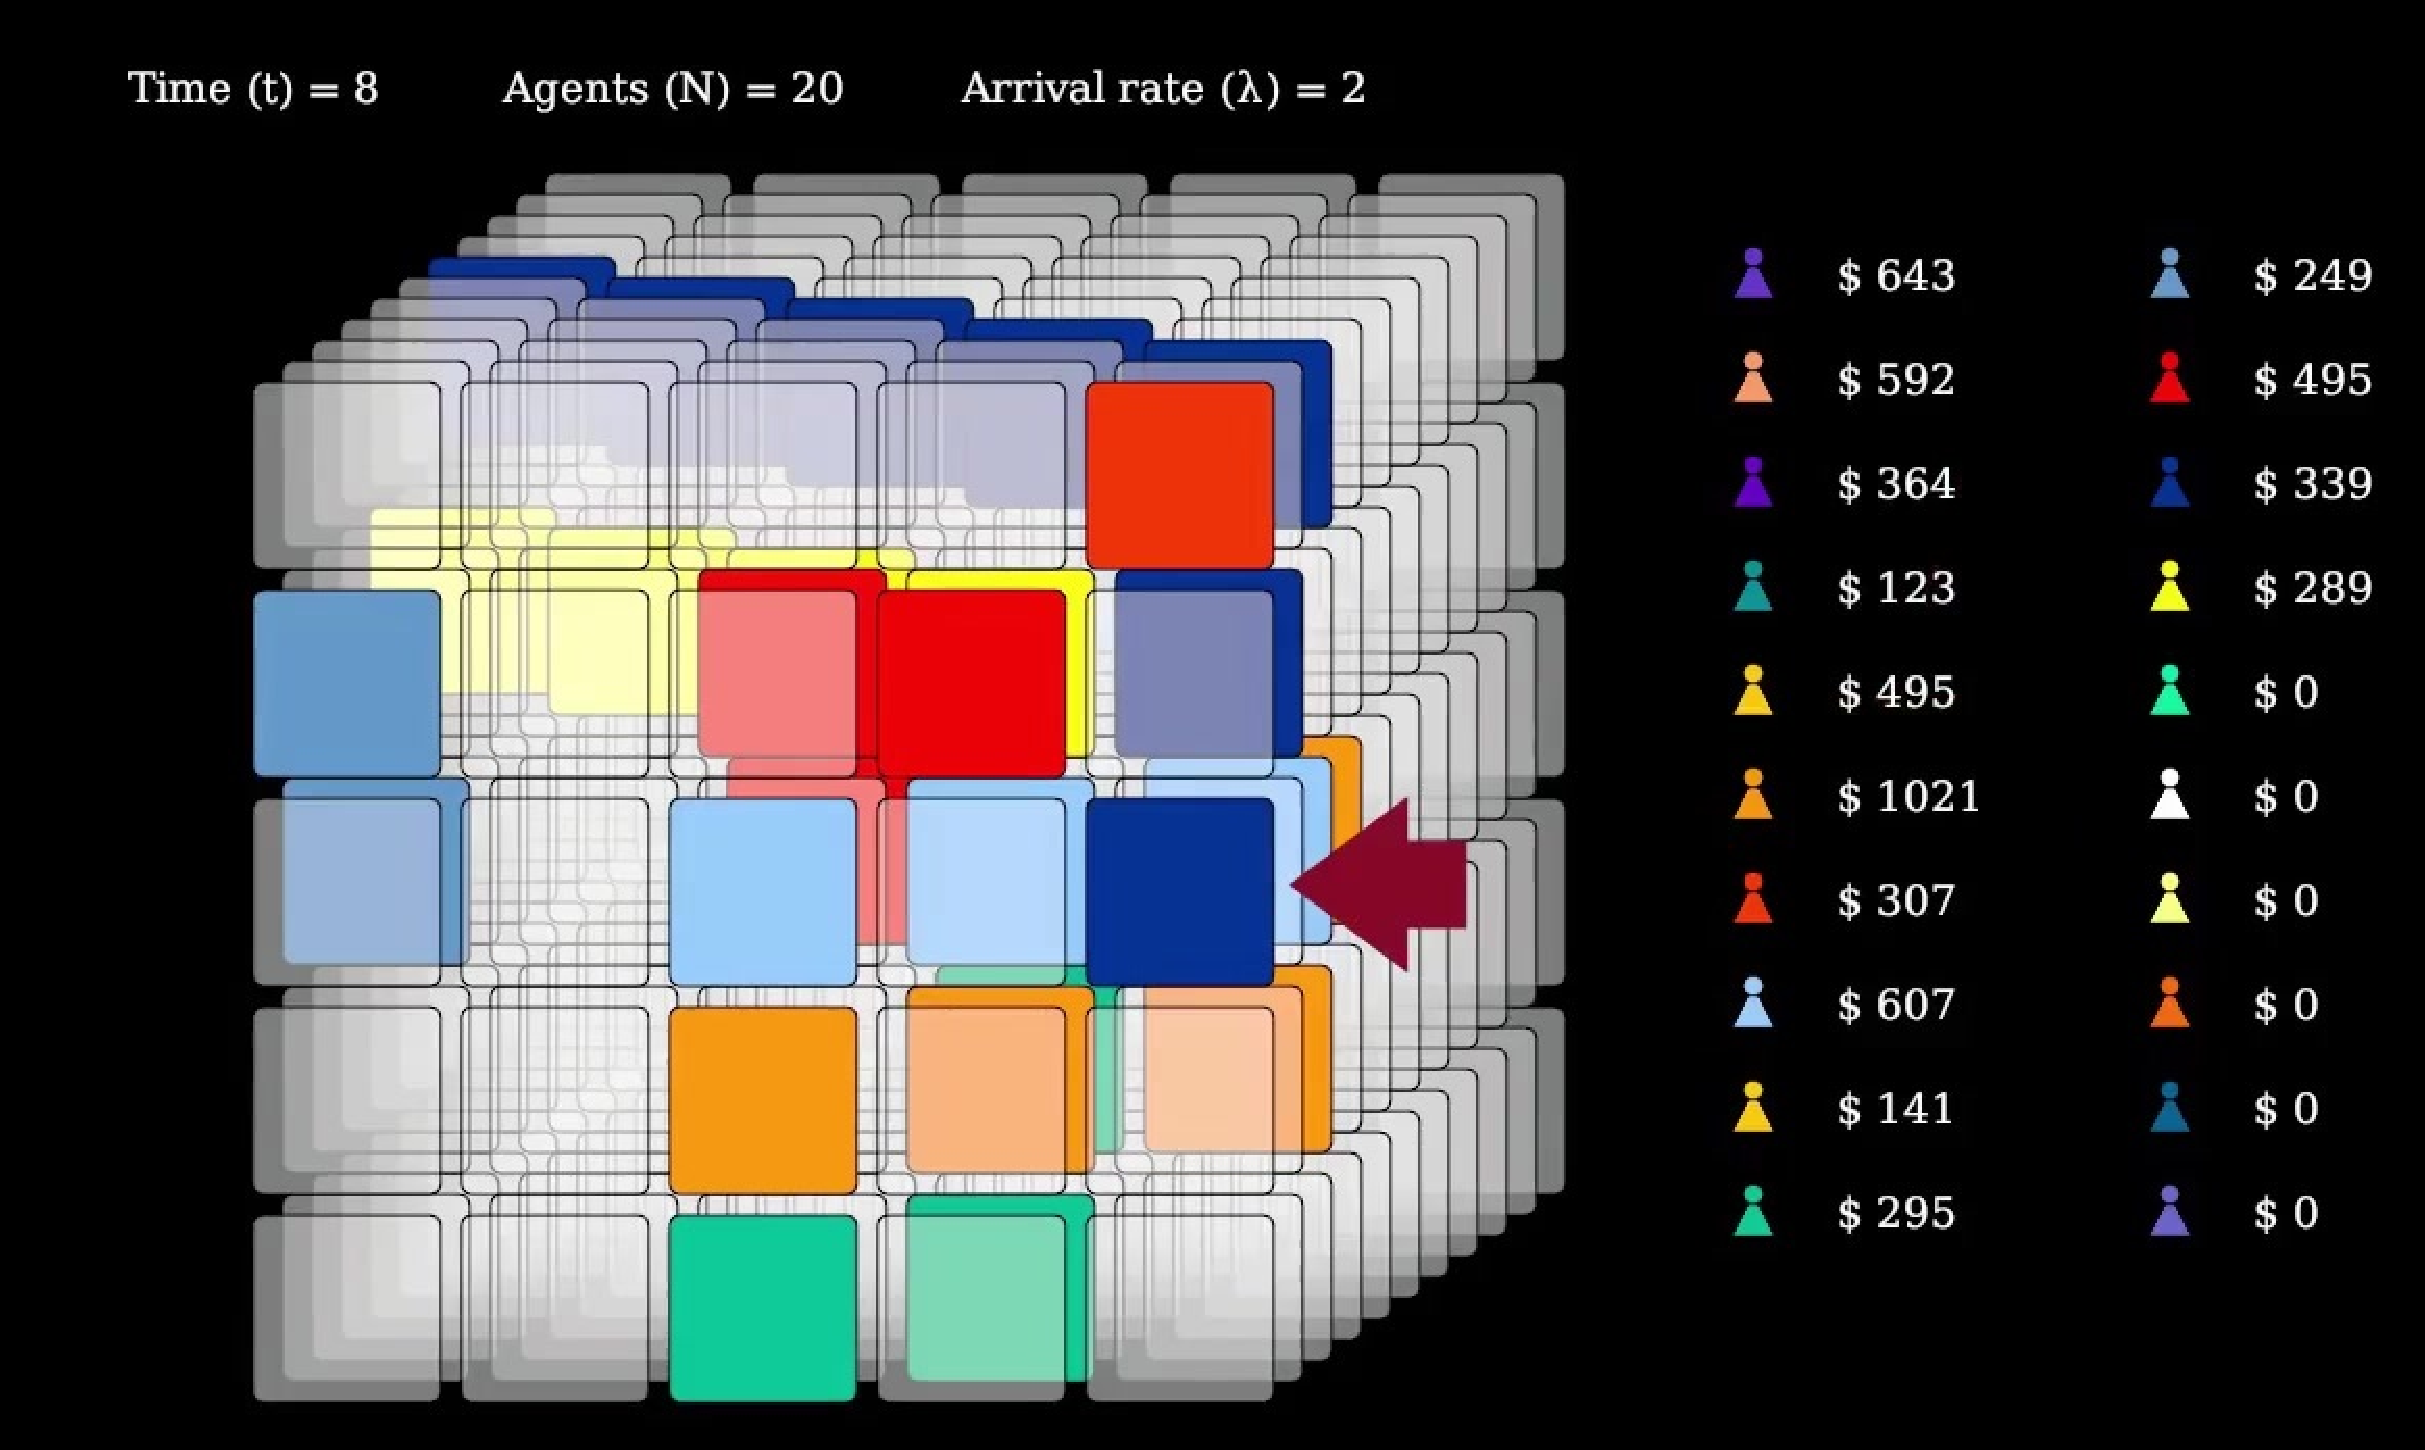
\includegraphics[width=\textwidth]{img/trad_drones-pdf-jpg-to-pdf.pdf}
      \end{columns}
    \end{figure}

\end{frame}


\begin{frame}{Future Works}
\destaq{Decentralized Model from \cite{Verri}}
\begin{itemize}
    \item naive agents
    \item greedy random choices
\end{itemize}
\bigskip
\destaq{Decentralized Model with Intelligence}
\begin{itemize}
    \item Reinforcement Learning
    \item Graph Dynamical System
    \begin{itemize}
        \item Complex Networks
        \item Graph Neural Networks
    \end{itemize}
\end{itemize}
\end{frame}



%%%%%%%%%%%%%%%%%%%%%%%%%%%%
\section{References}

% \nocite{*}
\begin{frame}[allowframebreaks]
  \frametitle{References}
  \bibliographystyle{siam}
  
  \bibliography{refs.bib}
\end{frame}

\end{document}